\documentclass[10pt]{article}         %% What type of document you're writing.
\usepackage{graphicx}
\usepackage{hyperref}
\usepackage[dvipsnames]{xcolor}

%%%%% Preamble

%% Packages to use

\usepackage{amsmath,amsfonts,amssymb}   %% AMS mathematics macros

%% Title Information.

\title{Data Model}
\author{Leonardo Martinez}
%% \date{29 sep 2020}           %% By default, LaTeX uses the current date

%%%%% The Document

\begin{document}

\maketitle

\begin{abstract}
This document implements the Data Model.
\end{abstract}

\section{Data Model Desciption}

\begin{enumerate}

\item
The company is organized into departmen.\\
Each deparment has a unique \textcolor{green}{name}, a unique \textcolor{green}{number}\\
and a particular employee who \textcolor{yellow}{manages} the department.
we keep track of the \textcolor{green}{start date}when that employee began mangin the deparment\\
A deparment may have several \textcolor{green}{locations}

\item
A deparment \textcolor{yellow}{controls} a number of projects, each of whicj has a unique \textcolor{green}{name}, a unique \textcolor{green}{number}, and a single \textcolor{green}{locations}

\item
The database will store each employee’s \textcolor{green}{name},\textcolor{green}{Social Security number},\textcolor{green}{
address}, \textcolor{green}{salary}, \textcolor{green}{sex (gender)}, and \textcolor{green}{birth date}. 
\\
An employee \textcolor{yellow}{is assigned} to one
department, but may \textcolor{green}{work} on several projects, which are not necessarily
controlled by the same department. It is required to keep track of the cur-
rent \textcolor{green}{number of hours per week} that an employee works on each project
\\
***as well as the direct \textcolor{yellow}{supervisor} of each employee (who is another employee)***.

\end{enumerate}


\section{E-R Model}

Data Model ...
\begin{figure}[b]
     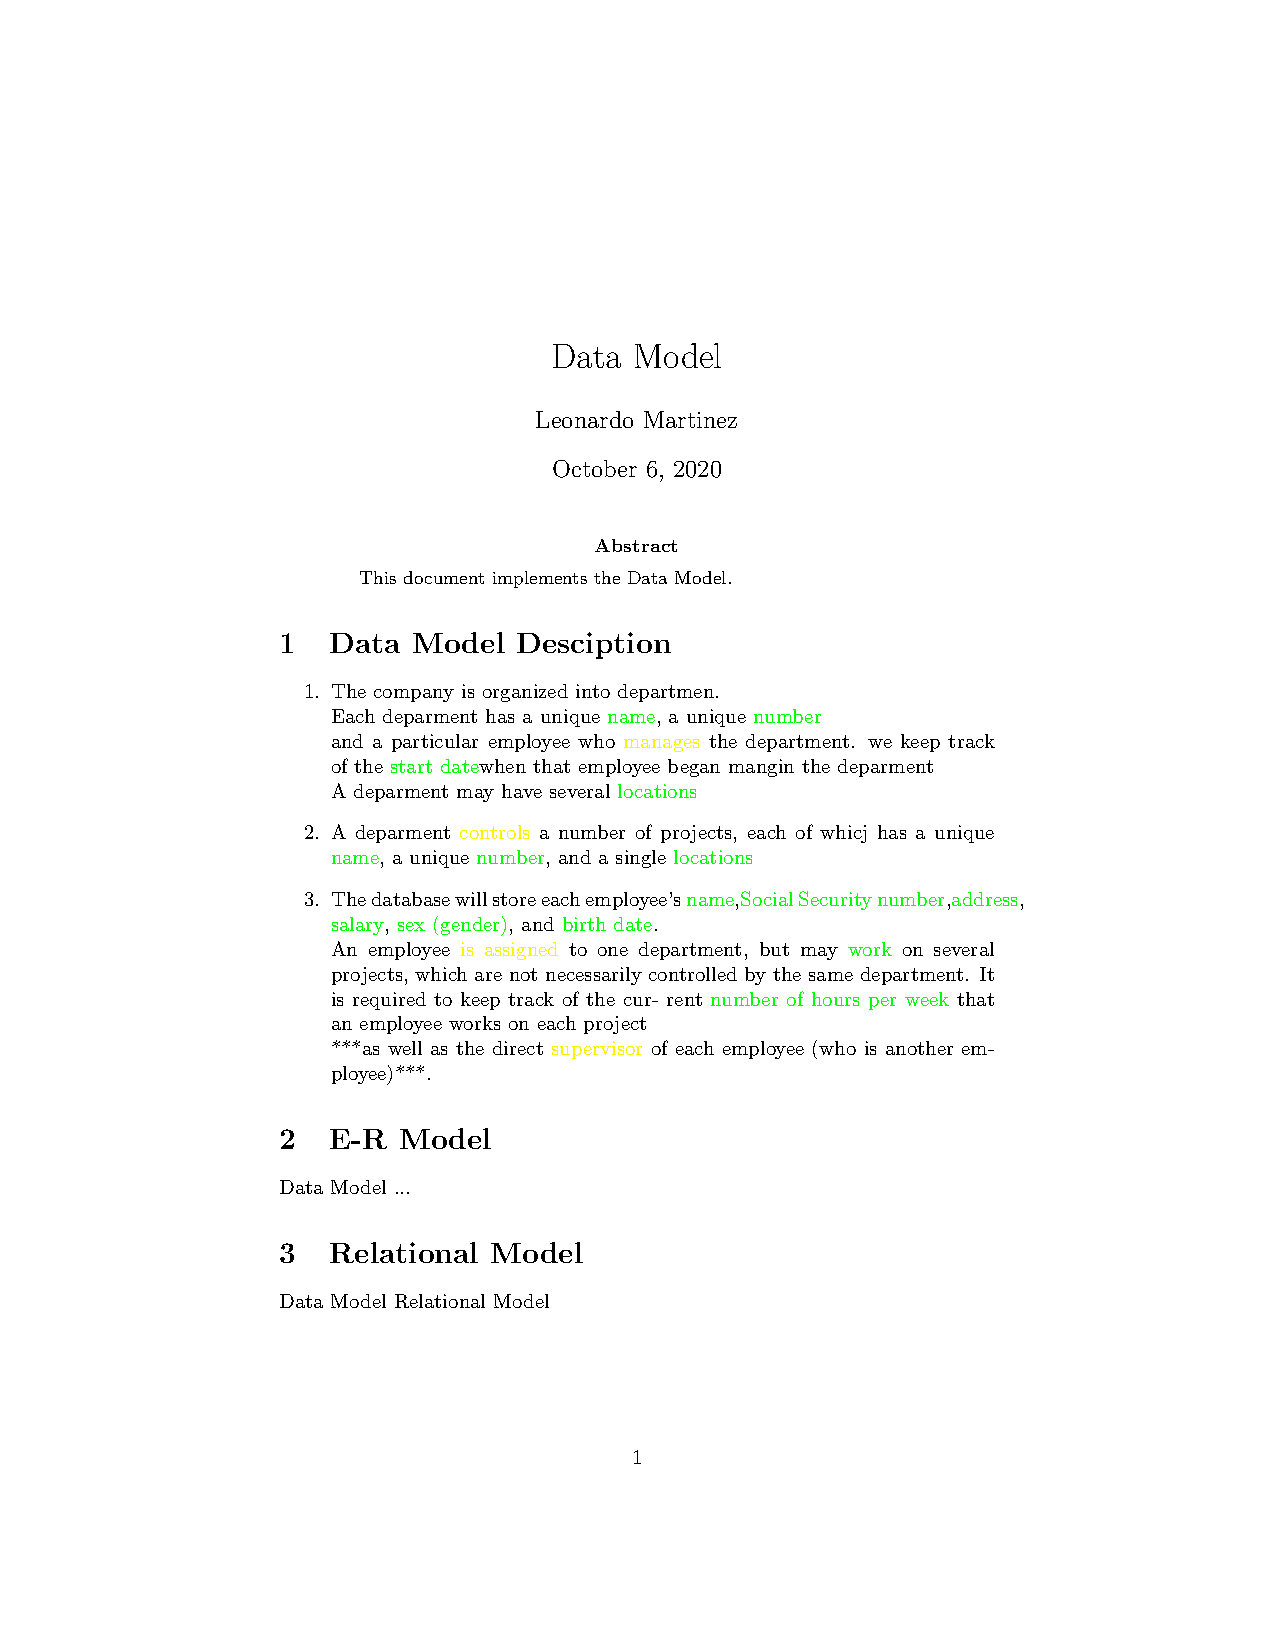
\includegraphics[scale=0.4]{data_model_er.png}
     \caption{data model E-R Model}
\end{figure}

\section{Relational Model}
Data Model  Relational Model

 \begin{figure}[b]
     \includegraphics[scale=0.4]{data_modePostgres.png}
     \caption{data model Relation Model}
\end{figure}

\section{Steps}

\begin{enumerate}

\item
sudo ssh -i leonardodmm leonardodmm@104.198.244.0
\item
sudo -u postgres createdb leonardodmm\_empresa
\item
\textbackslash connect leonardodmm\_empresa;
\item
create table employee (ssn int, bdate varchar(80),fname varchar(80),minit varchar,lname varchar(80),salary float,sex varchar(15),depnumber int,super\_ssn int);
\item
alter table employee  add constraint pk\_ssn primary key (ssn);
\item
alter table employee  add constraint fk\_super\_ssn foreign key(super\_ssn) references employee(ssn);
\item
create table dependent (dependt\_name varchar(100),sex varchar(15),bdate varchar(80),relationship varchar,essn int);
\item
alter table dependent add constraint fk\_essn foreign key(essn) references employee(ssn);
\item
create table department (number int,name varchar(120),mgr\_ssn int,dnumber int);
\item
alter table department add constraint pk\_number primary key(number);
\item
alter table department add constraint fk\_mgr\_ssn foreign key(mgr\_ssn) references employee(ssn);
\item
create table dept\_locations(dnumber int,location varchar);
\item
alter table dept\_locations add constraint pk\_dnumber primary key(dnumber);
\item
alter table department add constraint fk\_dnumber foreign key(dnumber) references dept\_locations(dnumber);
\item
 create table works\_on(ssn int,pnumber int,hours varchar(100));
\item
alter table works\_on add constraint fk\_ssn foreign key(ssn) references employee(ssn);
\item
create table project(pnumber int,pname varchar(200),plocation varchar,dnumber int);
\item
alter table project add constraint pk\_pnumber primary key(pnumber);
\item
alter table works\_on add constraint fk\_pnumber foreign key(pnumber) references project(pnumber);
\item
alter table project add constraint fk\_dnumber foreign key(dnumber) references department(number);
\item
alter table employee add constraint fk\_depnumber foreign key(depnumber) references department(number);




\end{enumerate}


\end{document}
